% Part: sets-functions-relations
% Chapter: infinite
% Section: hilberts-hotel
%
\documentclass[../../../include/open-logic-section]{subfiles}

\begin{document}

\olfileid{sfr}{infinite}{hilbert}
\olsection{Hilberts hotel}

De verzameling natuurlijke getallen is duidelijk oneindig. Als we de
natuurlijke getallen niet zonder meer \emph{als gegeven willen aannemen},
moeten we daarom eerst een oneindige verzameling karakteriseren zonder
de natuurlijke getallen zelf te noemen. Hilbert presenteerde hiervoor
in een voordracht uit 1924 een fraaie aanpak. Hij vraagt ons het
volgende voor te stellen:
\begin{quote}
[\ldots] een hotel met een eindig aantal kamers. Elk van deze kamers
dient door precies één gast bezet te zijn. Als de gasten nu op een of
andere manier van kamer wisselen, [maar] zodanig dat elke kamer nog
steeds hoogstens één persoon bevat, komen er geen kamers vrij en kan de
hoteleigenaar zo geen plaats maken voor een nieuw aangekomen gast [\ldots
\textparagraph \ldots]

Nu nemen we aan dat het hotel oneindig veel genummerde kamers $1$,
$2$, $3$, $4$, $5$, \dots{} heeft, die elk door precies één gast bezet
zijn. Zodra een nieuwe gast aankomt, hoeft de eigenaar slechts iedere
oude gast te verplaatsen naar de kamer met het nummer dat één hoger
ligt; kamer~$1$ is dan vrij voor de nieuw aangekomen gast.
	\begin{center}
		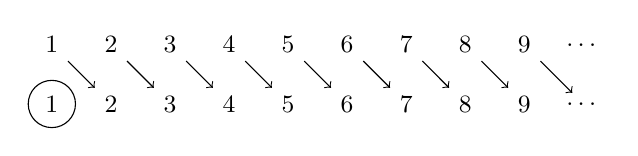
\begin{tikzpicture}[scale = .75]
		\foreach \x in {1, 2, 3, 4, 5, 6, 7, 8, 9}
		{
			\node (\x a) at (\x, 1) {\small{\x}};
			\node (\x b) at (\x, 2) {\small{\x}};
		}
		\node (dotsa) at (10, 1) {\small{\ldots}};
		\node (dotsb) at (10, 2) {\small{\ldots}};
		\draw[->] (1b)--(2a);
		\draw[->] (2b)--(3a);
		\draw[->] (3b)--(4a);
		\draw[->] (4b)--(5a);
		\draw[->] (5b)--(6a);
		\draw[->] (6b)--(7a);
		\draw[->] (7b)--(8a);
		\draw[->] (8b)--(9a);
		\draw[->] (9b)--(dotsa);
		\draw (1,1) circle (.4);
		\end{tikzpicture}
	\end{center}
	(gepubliceerd in \citealt[730]{EwaldSieg2013}; onze vertaling)
\end{quote}
Het wezenlijke punt is dat Hilberts hotel oneindig veel kamers heeft;
we kunnen zijn uitleg gebruiken om te definiëren wat dat betekent.
Dit was inderdaad Dedekinds aanpak (hier uiteraard op sterk
anachronistische wijze gepresenteerd; Dedekinds definitie dateert uit
\citeyear{Dedekind1888}):

\begin{defn}\ollabel{defn:DedekindInfinite}
Een verzameling $A$ is \emph{Dedekind-oneindig} dan en slechts dan als
er een injectie van~$A$ naar een echte deelverzameling van~$A$ bestaat.
Dat wil zeggen: er bestaan een $o \in A$ en een injectie $f \colon A
\to A$ zodanig dat $o \notin \ran{f}$.
\end{defn}

\end{document}